Imagine a high-speed train approaching a busy platform. In the critical seconds before the train comes to a complete stop and doors open, it is operationally valuable for the driver and the onboard control system to anticipate the number of passengers waiting on the platform. Such foresight directly informs precise dispatching strategies and efficient boarding/alighting\cite{214,215,216}.

For railway operators, obtaining real-time situational awareness of platform crowds during train approach is essential to intelligent dispatch and proactive safety assurance\cite{214,215,216}. A vision system mounted on the train head can provide this “look-ahead” capability, transforming traditional passive platform monitoring into active, forward-looking risk assessment and operational decision-making.

\subsection{Objective}

Our objective is to use a camera mounted at the train head to detect, track, and uniquely count passengers on the platform in real time throughout the approach phase.

\subsection{Challenges}

\subsubsection{Challenge 1: Detection under extreme perspective changes and occlusion}
As the train approaches at speed, the camera undergoes large perspective changes: distant heads rapidly scale up and apparent motion is highly non-linear. Severe mutual occlusions inherent to dense crowds further degrade full-body detectors (e.g., YOLO variants), leading to instability and missed detections due to motion blur and heavy overlap\cite{29_kaur_systematic_2024,30_khan_passenger_2020,01_noauthor_deep_2024,66_zhang_bus_2020,33or34_li_lightweight_2023}.

\subsubsection{Solution 1: Robust head-based detection}
To mitigate these effects, we shift the detection target from full bodies to heads, which remain more visible at high density and under occlusion. Leveraging public datasets (CrowdHuman, Open Sensor Data for Rail 2023, RailEye3D) and our domain-specific RailwayPlatformCrowdHead dataset, we fine-tune a YOLOv11m detector via two-stage transfer learning\cite{shao2018crowdhuman,OpenSensorDataforRail2023,RailEye3D_Dataset}. The model is specialized for head cues from the train viewpoint and is robust to extreme scale variation and perspective distortion; the YOLO family is widely adopted for real-time detection\cite{02_noauthor_review_nodate,141}.

\subsubsection{Challenge 2: Tracking degradation due to ego-motion}
A central difficulty in multi-object tracking (MOT) is predicting targets’ next-frame states\cite{104,103}. Under fast ego-motion, classical motion models such as constant-velocity (8D) or constant-acceleration (12D) Kalman filters confound real target motion with apparent motion induced by camera movement, yielding physically inconsistent trajectories and frequent identity switches (ID switches).

\subsubsection{Solution 2: A physics-constrained model with ego-motion integration}
We propose Phys-5D, a five-dimensional Kalman variant that integrates the train’s ego-motion as prior knowledge in state prediction. Operating in a perspective-aware coordinate system with geometric constraints, Phys-5D decouples true target motion from apparent motion induced by camera advance. This significantly stabilizes trajectory predictions during rapid approach, reduces identity fragmentation, and preserves a compact state representation.

\subsubsection{Challenge 3: Converting dynamic tracks into reliable counts}
Even with stable tracking, converting rapidly evolving image-plane tracks into reliable, region-specific counts (e.g., per-car boarding zones) is nontrivial. Short occlusions and detection jitter can interrupt tracks, causing duplicates or misses for naive counting logic.

\subsubsection{Solution 3: Geography-anchored virtual counting zones}
We introduce geography-anchored virtual counting regions corresponding to real platform locations. Stabilized tracks are mapped to these zones with a temporal persistence window to absorb brief interruptions and positional jitter. 

\subsection{Results}
With domain-adaptive fine-tuning for the train-view setting, the head detector achieves a substantial accuracy gain: $mAP_{50}$ increases from 79.4\% to \textbf{98.0\%}, and $mAP_{50\text{--}95}$ from 54.7\% to \textbf{81.6\%}. On the \textbf{MOT-RPCH} benchmark built for this scenario, Phys-5D attains a \textbf{2.24\%} mean absolute percentage error (MAPE) in counting, surpassing constant-velocity (14.59\%) and constant-acceleration (6.99\%) baselines. It maintains \textbf{67\%} MOTA while substantially reducing identity switches. Combined with an EfficientNet-B0 appearance encoder, the system reliably restores identities after long occlusions from poles or other structures.

\subsection{Contributions}
In summary, our main contributions are:
\begin{itemize}
    \item We design a real-time, end-to-end \textbf{detect–track–analyze} pipeline tailored for train approach, enabling forward-looking platform perception onboard the train\cite{113,28_kaur_comprehensive_2023}.
    \item We propose a \textbf{Phys-5D Kalman filter} that incorporates physically grounded ego-motion constraints to address instability under strong perspective and camera motion.
    \item We release a new domain-specific dataset, \textbf{RailwayPlatformCrowdHead}, to facilitate head-based detection and crowd analytics from the train viewpoint.
    \item We demonstrate that combining physics-based motion modeling with deep visual representation yields \textbf{accurate, stable, and efficient} solutions for physically constrained vision tasks in transportation; for tracking-by-detection and DeepSORT foundations see\cite{132,211,212}.
\end{itemize}

\subsection{Preview}
Fig.~\ref{fig:intro_preview1} and Fig.~\ref{fig:intro_preview2} shows frames from a tracked video sequence, indicating currently tracked objects with their unique IDs and the unique-ID count from the virtual counting zone displayed at the bottom-left.
\begin{figure}[htbp]
    \centering
    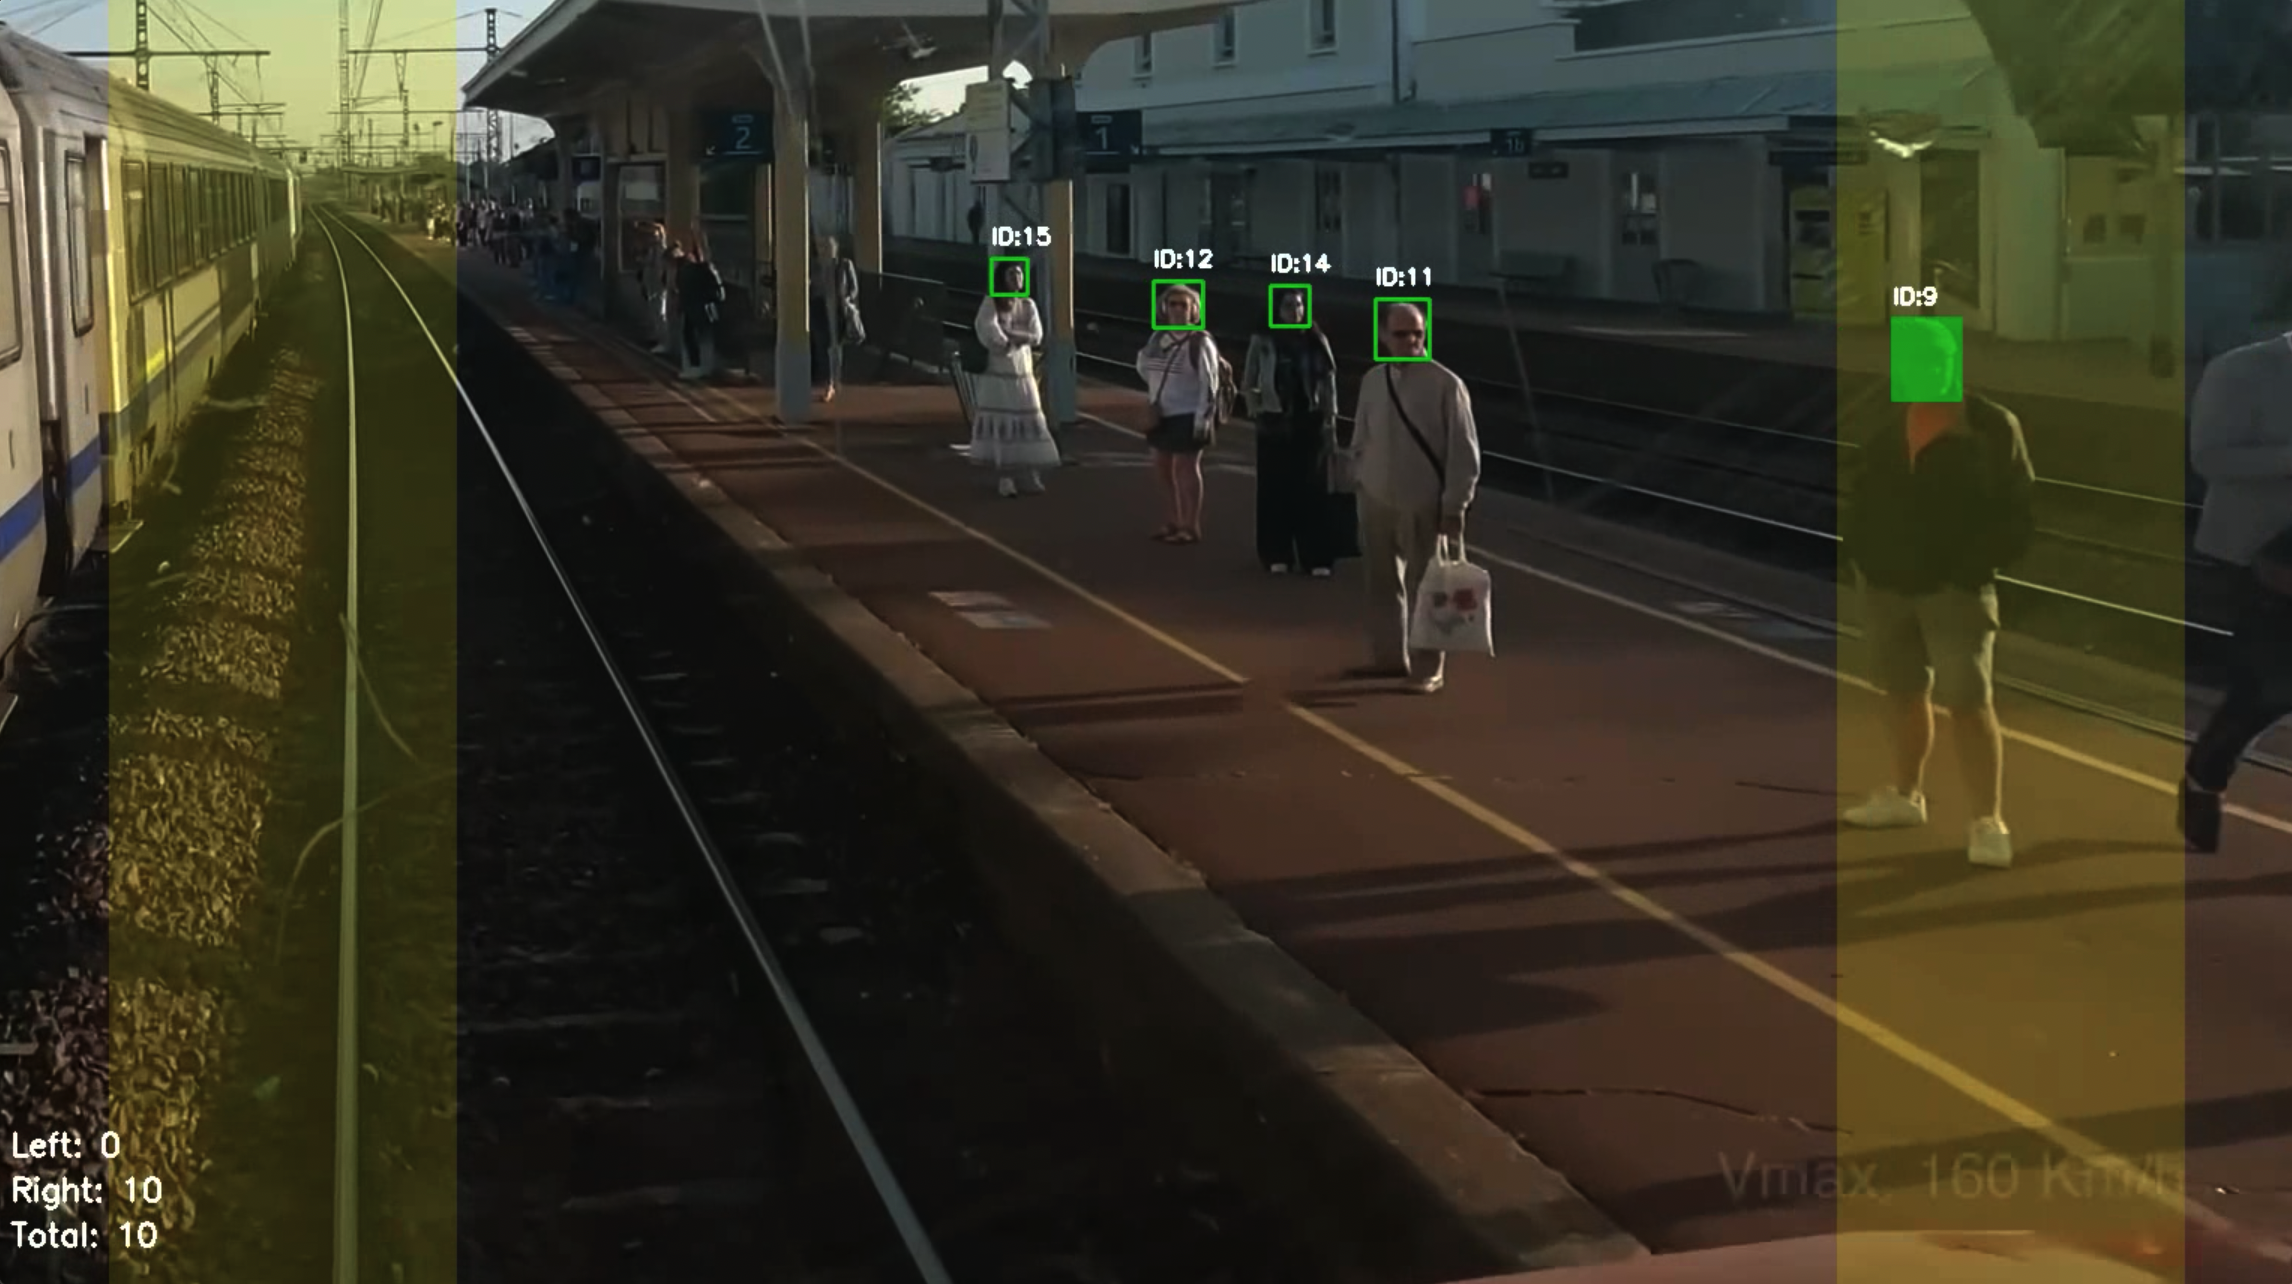
\includegraphics[width=0.49\textwidth]{pictures/Phys5Dframedeomo.png}  
    \caption{Frames from a tracked video sequence. Each bounding box is annotated with a unique track ID:9,11,14,12,15; the bottom-left overlay shows the unique-ID count(Total:10) from the virtual counting zone(yellow area).}
    \label{fig:intro_preview1}
\end{figure}

\begin{figure}[htbp]
    \centering
    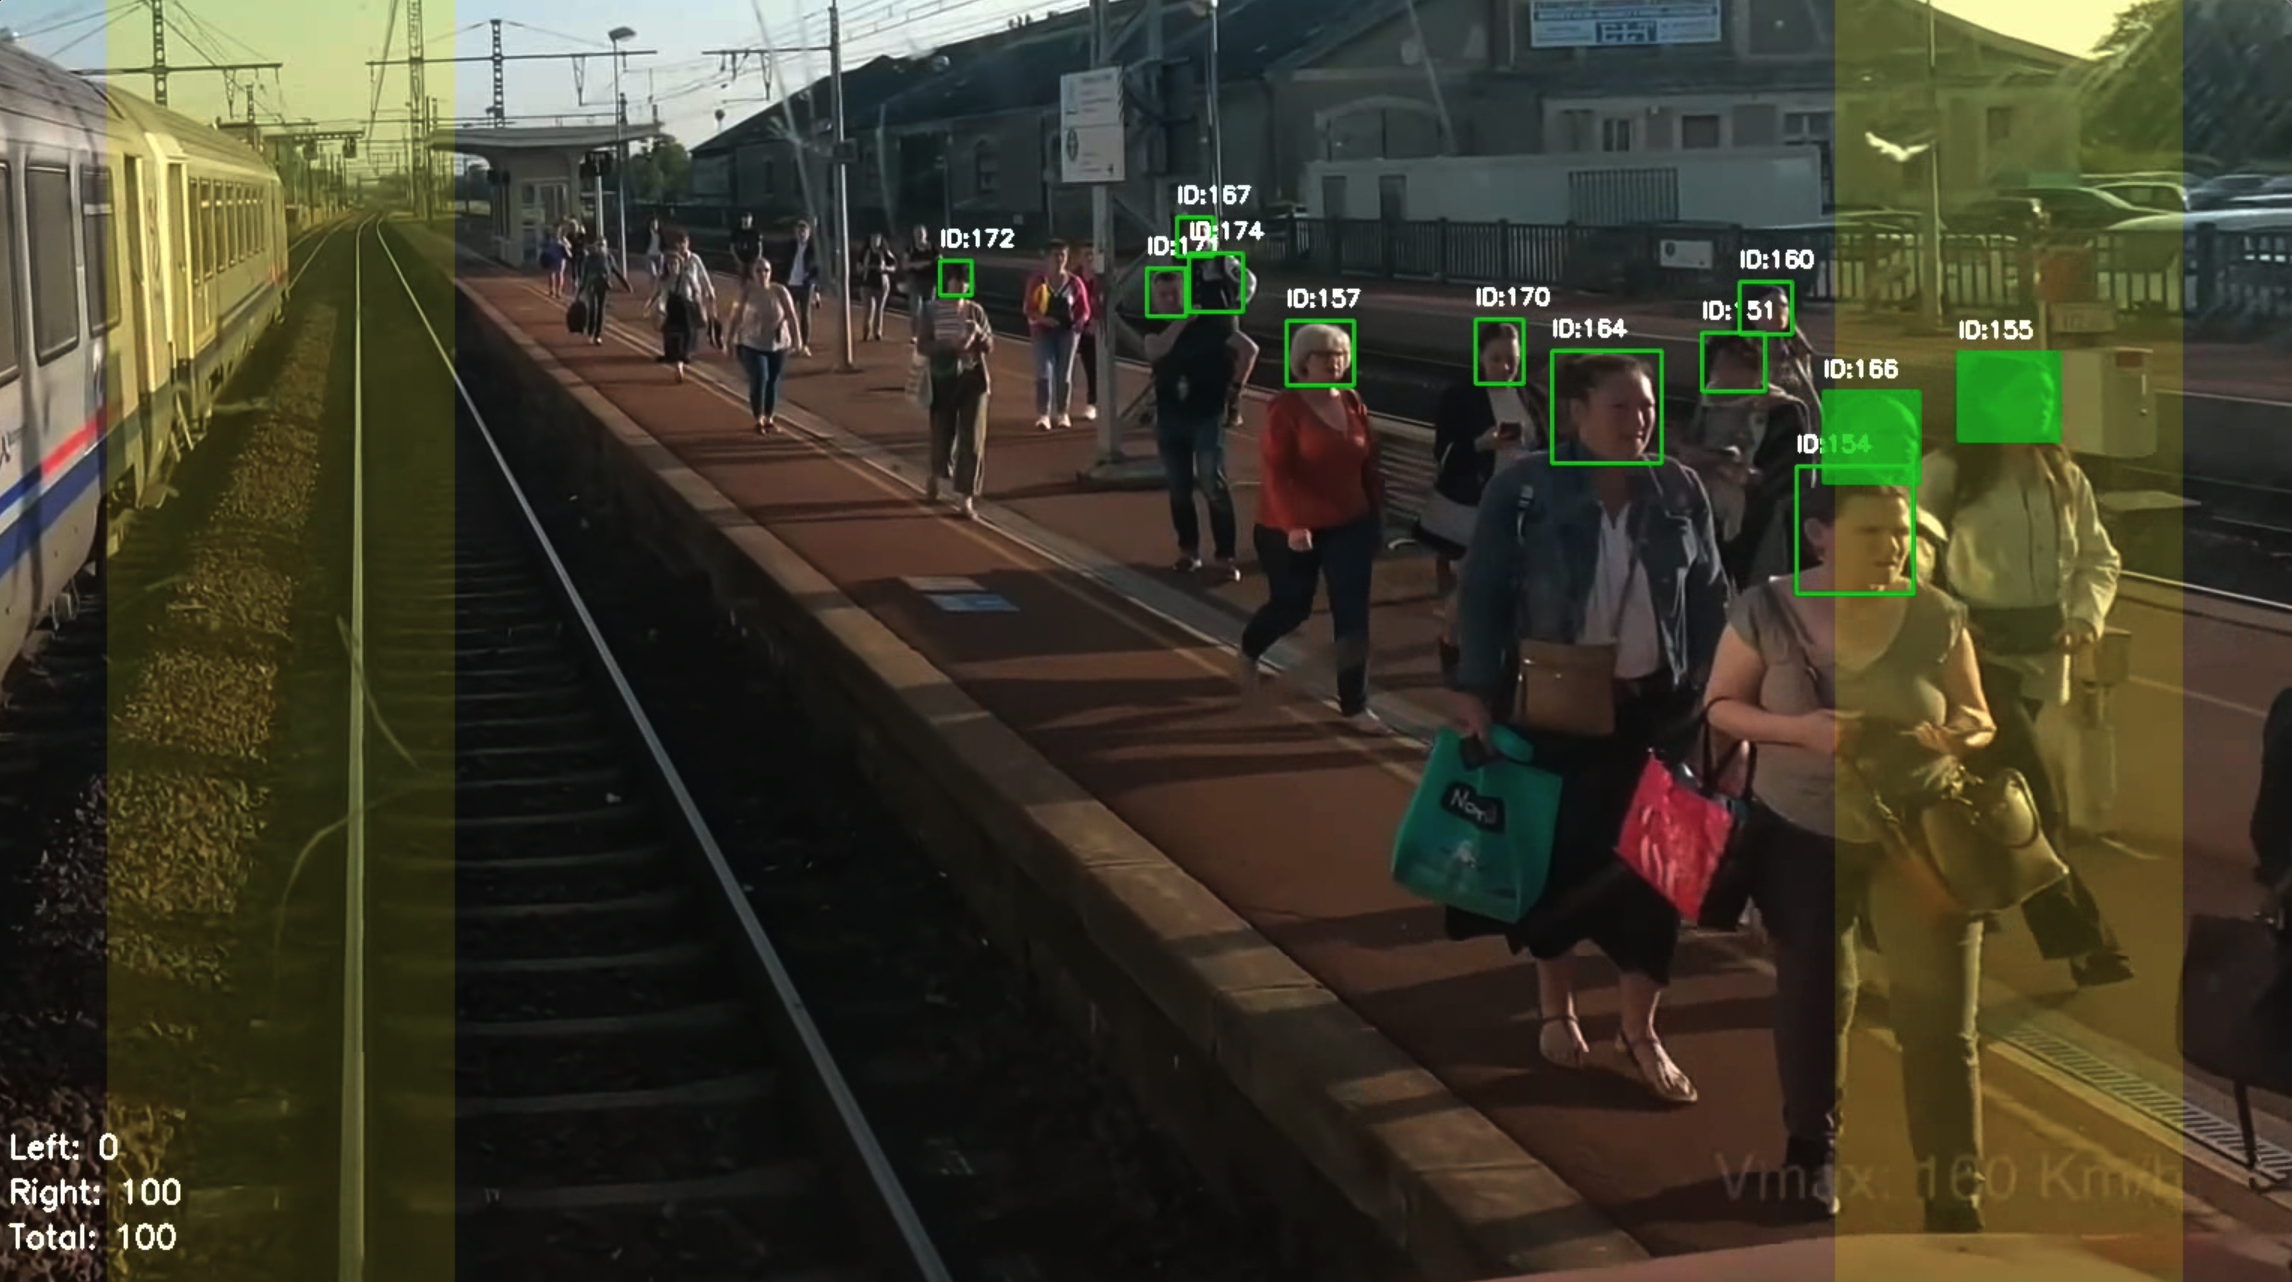
\includegraphics[width=0.49\textwidth]{pictures/Phys5Dframedeomo2.png}  
    \caption{Frames from a tracked video sequence. Each bounding box is annotated with a unique track ID:154,155,166 ...; the bottom-left overlay shows the unique-ID count(Total:100) from the virtual counting zone(yellow area).}
    \label{fig:intro_preview2}
\end{figure}
